\subsection{Пример работы программы}

Для примера снова обратимся к модели электродвигателя постоянного тока, рассмотренной в разделе \ref{sec:continuous-example}. Будем предполагать, что управление запаздывает на $h = 0,\!05$, а интервал между наблюдениями $\varepsilon = 0,\!2$.

Переведём систему \eqref{eq:x-example} к дискретному виду. Матрицы посчитаны численными методами. Получим систему
\begin{equation}\label{eq:ex-discr-sys}
x^{k+1} = \Phi x^k + \Gamma_1 u^k + \Gamma_2 u^{k-1},
\end{equation}
где
$$
        \Phi = e^{A\varepsilon} \approx \begin{pmatrix}
\;\;\,0,\!6705 & -0,\!0013 \\
-0,\!0669 & \;\;\,0,\!1354
        \end{pmatrix},
$$
$$
        \Gamma_1 = \int\limits_{h}^{\varepsilon}
        e^{As}\,ds \cdot B \approx
\begin{pmatrix}
\;\;\,0,\!2345 \\
-0,\!0175
\end{pmatrix}, 
$$
$$
        \Gamma_2 = \int\limits_{0}^{h}
        e^{As}\,ds \cdot B \approx
        \begin{pmatrix}
\;\;\,0,\!0952 \\
-0,\!0021
        \end{pmatrix}.
$$
Убедиться в том, что построенный перевод верен можно на Рис.~\ref{img:cont-and-disc}.
\begin{figure}[h]
        \noindent\centering{
        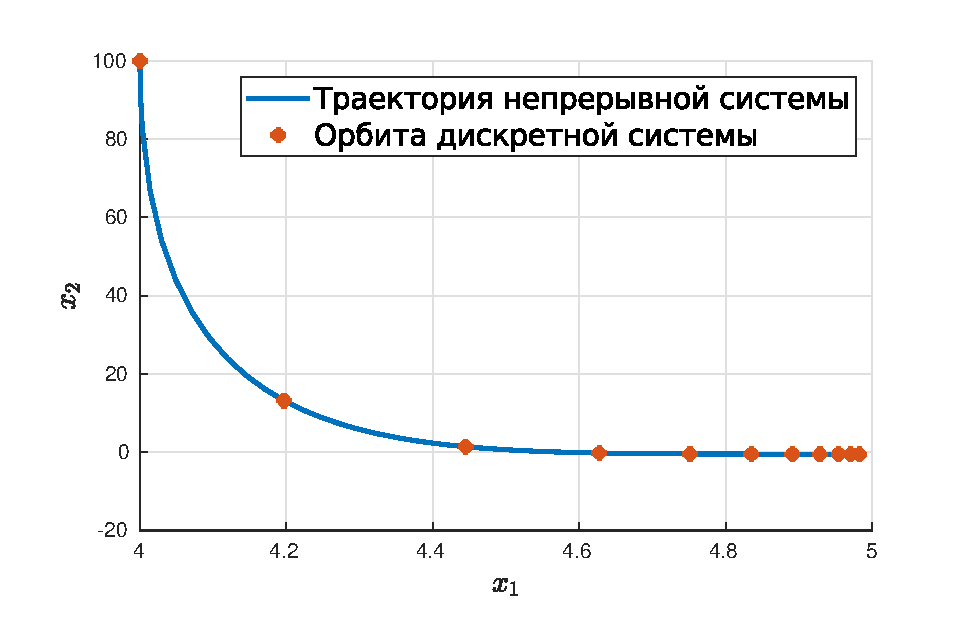
\includegraphics[width=160mm]{content/discrete_task/example/cont-and-disc.eps}
        }
        \caption{Траектория непрерывной системы~\eqref{eq:x-example} и орбита соответствующей редуцированной дискретной системы~\eqref{eq:ex-discr-sys}, выпущенной из начальной точки $x_0 = [4,\, 100]\T$ с постоянным управлением $u \equiv 1$.
        }
        \label{img:cont-and-disc}
\end{figure}

Приведем пример работы программы для параметров задачи \eqref{eq:ex-mat}, \eqref{eq:ex-start}, которые мы использовали в разделе \ref{sec:continuous-example}. На Рис.~\ref{img:discr-control} представлено соответствующее решение дискретной задачи. На Рис.~\ref{img:control}, Рис.~\ref{img:ex-discr-coords} представлено управление, действующее на управляемый объект и соответствующая траектория.

\begin{figure}[bh]
        \noindent\centering{
        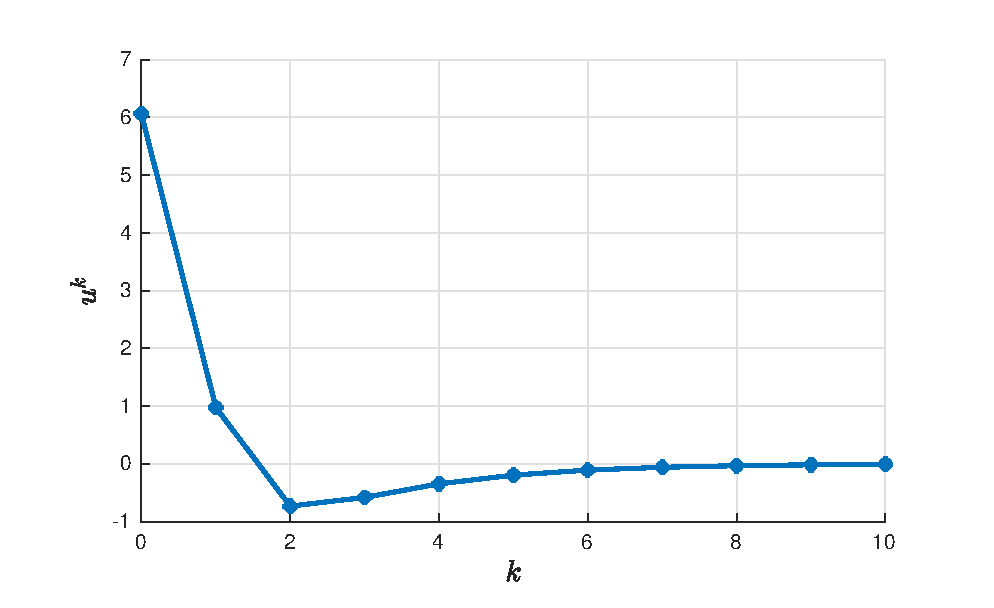
\includegraphics[width=160mm]{content/discrete_task/example/discr_control.eps}
        }
        \caption{Оптимальное управление дискретной системой~\eqref{eq:ex-discr-sys}.}
        \label{img:discr-control}
\end{figure}
\begin{figure}[bh]
        \noindent\centering{
        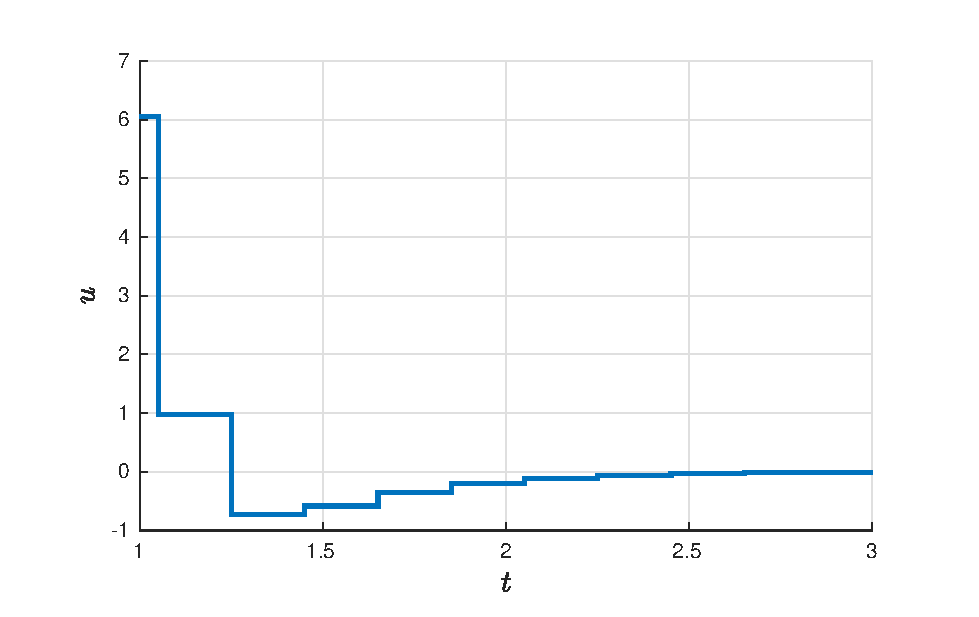
\includegraphics[width=160mm]{content/discrete_task/example/control.eps}
        }
        \caption{Управление, действующее на объект, при использовании оптимальной стратиегии Рис.~\ref{img:discr-control}.}
        \label{img:control}
\end{figure}
\begin{figure}[bh]
        \noindent\centering{
        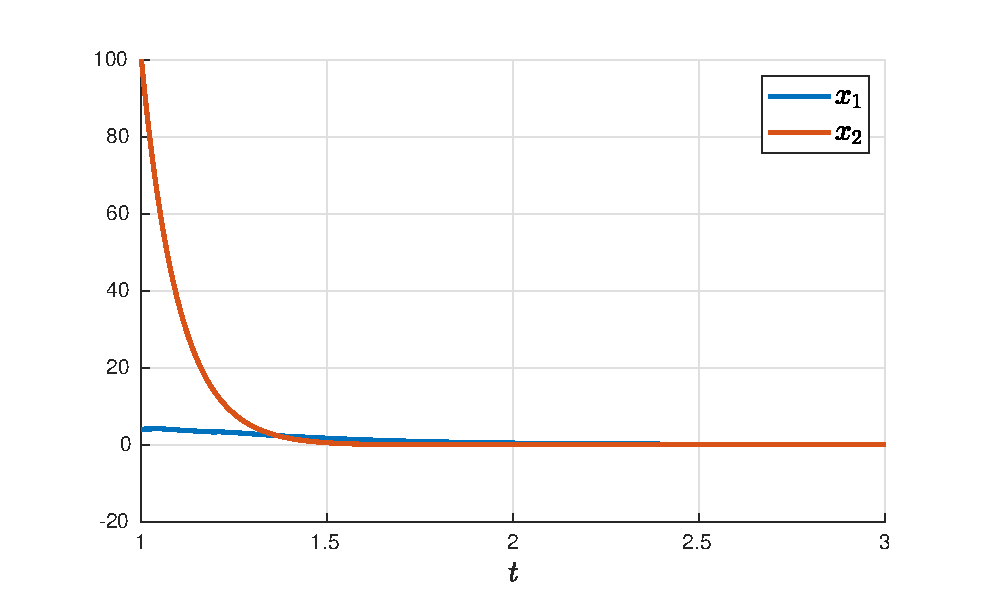
\includegraphics[width=160mm]{content/discrete_task/example/coords.eps}
        }
        \caption{Поведение системы~\eqref{eq:x-example} при передаче управления Рис.~\ref{img:control}.}
        \label{img:ex-discr-coords}
\end{figure}

При уменьшении интервала между известными состояниями $\varepsilon$ можно использовать построенный алгоритм для решения непрерывной задачи. Для сравнения с построенным ранее управлением Рис.~\ref{img:small-control} приведем на Рис.~\ref{img:ex-small-control} пример работы программы для $h = 0,\!5$, $\varepsilon = 10^{-2}$. В отличие от непрерывного алгоритма, время подсчета текущего состояния объекта не зависит от величины запаздывания. Эта часть в обоих алгоритмах выполняется на каждой итерации работы программы. Значит, второй способ должен работать быстрее при большой величине запаздывания. Сравнение времени работы каждой из программ представлено на Рис.~\ref{img:cpu}.

\begin{figure}[bh]
        \noindent\centering{
        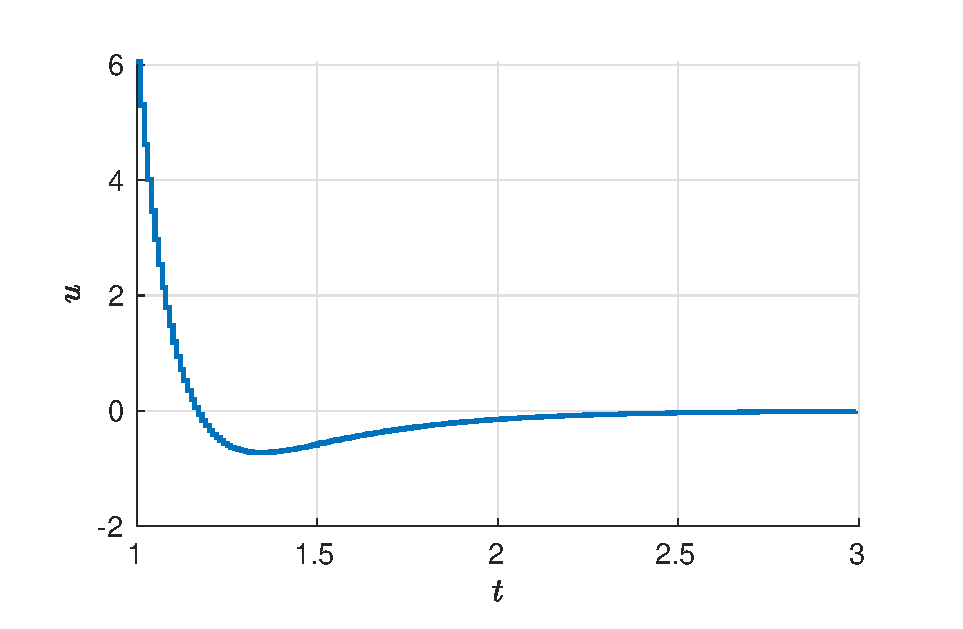
\includegraphics[width=160mm]{content/discrete_task/example/small-control.eps}
        }
        \caption{.}
        \label{img:ex-small-control}
\end{figure}
\begin{figure}[bh]
        \noindent\centering{
        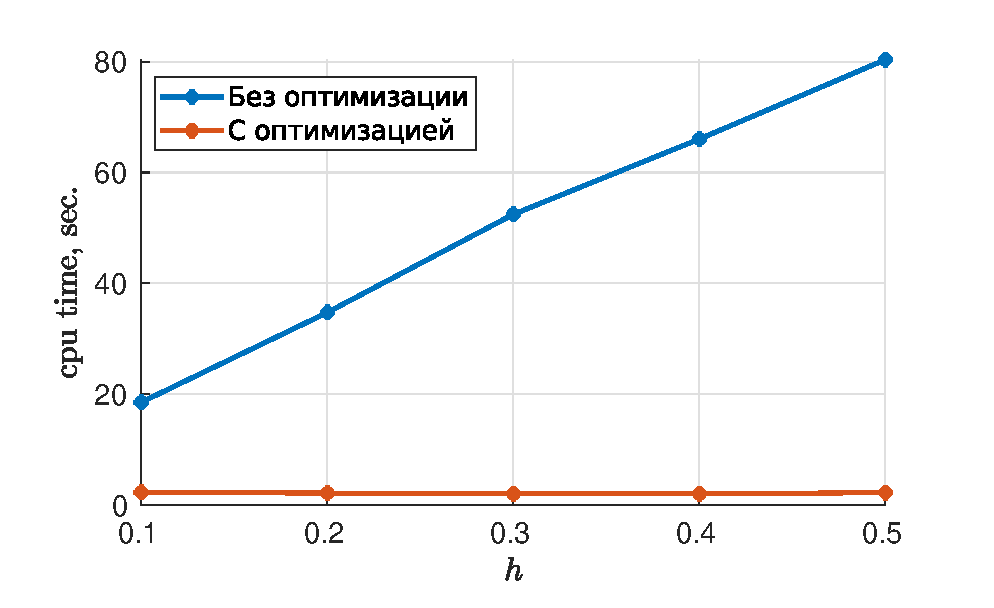
\includegraphics[width=160mm]{content/discrete_task/example/cpu.eps}
        }
        \caption{.}
        \label{img:cpu}
\end{figure}